\documentclass[a4paper,oneside,12pt]{book}

% Variable definitions
\newcommand{\thesistitle}{HubSpot Software Engineering Internship} % Your thesis title, this is used in the title and abstract
\newcommand{\degree}{MAI (Computer Engineering)} % Your degree name, this is used in the title page and abstract
\newcommand{\typeofthesis}{Internship Report} % dissertation, Final Year Project, report, etc.
\newcommand{\authorname}{Stefano Lupo} % Your name, this is used in the title page and PDF stuff
\newcommand{\authorid}{14334933} % Your ID
\newcommand{\keywords}{HubSpot, Software Engineering, Programming, Computer Engineering, 4E4 Internship} % Keywords for your thesis
\newcommand{\school}{\href{http://www.scss.tcd.ie}{School of Computer Science and Statistics}} % title page

\title{\thesistitle}
\author{\authorname}

% Configure output pdf properties
\AtBeginDocument{
\hypersetup{pdftitle=\thesistitle}
\hypersetup{pdfauthor=\authorname}
\hypersetup{pdfkeywords=\keywords}
\hypersetup{pdfsubject=\degree}
}

% Language and font encodings
\usepackage[T1]{fontenc} 
\usepackage[utf8]{inputenc}
\usepackage[english]{babel}

% Bibliographical stuff
\usepackage[round,sort,comma,numbers]{natbib}

% Document size
% include showframe as an option if you want to see the boxes
\usepackage[a4paper,top=2.54cm,bottom=2.54cm,left=2.54cm,right=2.54cm,headheight=16pt]{geometry}
\pagestyle{plain} % Embrace simplicity!

% Useful packages
\usepackage{amsmath}
\usepackage[autostyle=true]{csquotes} % Required to generate language-dependent quotes in the bibliography
\usepackage[pdftex]{graphicx}
\graphicspath{{./assets/}}
\usepackage[colorinlistoftodos]{todonotes}
\usepackage[colorlinks=true, allcolors=black]{hyperref}
\usepackage{caption} % if no caption, no colon
\usepackage{sfmath} %use sans-serif in the maths sections too
\usepackage[parfill]{parskip}    % Begin paragraphs with an empty line rather than an indent
\usepackage{setspace} % to permit one-and-a-half or double spacing
\usepackage{enumerate} % fancy enumerations like (i) (ii) or (a) (b) and suchlike
\usepackage{booktabs} % To thicken table lines
\usepackage{fancyhdr}

%%%%%%%%%%%%%%%%%%%%%%%%%%%%%%%%%%%%%%%%%%%%%%%%%%%%%%%%%%%%%%%%%%%%%%%%
% My Packages
\usepackage{enumitem} %Nested lists a la TOC (plan)
\setlist[enumerate]{label*=\arabic*.}

\usepackage{scrextend}  % List with description all descriptions tabbed as wide as longest
\addtokomafont{labelinglabel}{\sffamily} % Who knows what this does

\usepackage{listings} % Code listing
\definecolor{dkgreen}{rgb}{0,0.6,0}
\lstdefinestyle{javaStyle} {
  language=Java,
  aboveskip=5mm,
  belowskip=5mm,
  showstringspaces=false,
  columns=flexible,
  basicstyle={\footnotesize\ttfamily},
  numberstyle={\tiny},
  numbers=left,
  keywordstyle=\color{blue},
  commentstyle=\color{dkgreen},
  stringstyle=\color{gray},
  breaklines=true,
  breakatwhitespace=true,
  tabsize=2
}

\usepackage{float} % Figure placement

\usepackage{xcolor}

\usepackage[toc,page]{appendix}
\renewcommand{\appendixname}{Annex}

%%%%%%%%%%%%%%%%%%%%%%%%%%%%%%%%%%%%%%%%%%%%%%%%%%%%%%%%%%%%%%%%%%%%%%%
% Custom commands
\newcommand{\team}{Email Sending Infrastructure}
\newcommand{\sneaktitle}[1]{\hfill\break\break\textbf{#1}\hfill\break}
\newcommand{\refcode}[1]{code listing \ref{#1}}
\newcommand{\refsec}[1]{section \ref{#1}}
\newcommand{\refeq}[1]{equation \ref{#1}}
\newcommand{\reftbl}[1]{table \ref{#1}}
\newcommand{\reffig}[1]{figure \ref{#1}}
\newcommand{\refapp}[1]{appendix \ref{#1}}
\newcommand{\java}[1]{\fcolorbox{gray}{gray!50}{\lstinline{#1}}}
\newcommand{\sub}[1]{_\text{#1}}
%%%%%%%%%%%%%%%%%%%%%%%%%%%%%%%%%%%%%%%%%%%%%%%%%%%%%%%%%%%%%%%%%%%%%%%%

%%%%%%%%%%%%%%%%%%%%%%%%%%%%%%%%%%%%%%%%%%%%%%%%%%%%%%%%%%%%%%%%%%%%%%%%


% Default to Sans-Serif
\renewcommand{\familydefault}{\sfdefault}

% Options: Sans-Serif, Computer Modern(latex default), palatino
\usepackage{mathpazo} % math fonts
\usepackage{palatino} % nicer font

% Use continuous equation numbers
\renewcommand{\theequation}{\arabic{equation}} 

% Format Chapter headings appropriately
\usepackage{titlesec}
\titleformat{\chapter}[block] 
{\normalfont\huge\bfseries}{\thechapter}{0.6cm}{} 

\usepackage{titlesec}
\titleformat{\section}[block] 
{\normalfont\Large\bfseries}{\thesection}{0.6cm}{} 

\usepackage{titlesec}
\titleformat{\subsection}[block] 
{\normalfont\large\bfseries}{\thesubsection}{0.6cm}{} 

\frontmatter
\begin{document}
\begin{titlepage}

\center % Center everything on the page

%% All the text parameters should be taken from the start of the main.tex file.
%% You should only alter stuff here if you want to change the layout

%----------------------------------------------------------------------------------------
%	LOGO SECTION
%----------------------------------------------------------------------------------------
%% Choose one of the following -- a colour or black-and-white logo


\includegraphics{assets/Trinity_RGB_transparent_main.png}\\[1cm] 
%
\includegraphics[width=12cm]{title/black-stacked-trinity.jpg}\\[1cm] 

\Large \school\\[1.5cm] % Minor heading such as course title
\ifdefined\department
\large \department\\[1.5cm] % Minor heading such as course title
\fi

%----------------------------------------------------------------------------------------
%	TITLE SECTION
%----------------------------------------------------------------------------------------
\makeatletter
{ \huge \bfseries \thesistitle}\\[1.5cm] % Title of your document
 

%----------------------------------------------------------------------------------------
%	AUTHOR SECTION
%----------------------------------------------------------------------------------------

\ifdefined\authorid
\authorname\\ % Your name
\authorid\\[2cm] % Your Student ID
\else
\authorname\\[2cm] % Your name
\fi

%----------------------------------------------------------------------------------------
%	DATE SECTION
%----------------------------------------------------------------------------------------

{\large \today}\\[2cm] % Date, change the \today to a set date if you want to be precise

 
%----------------------------------------------------------------------------------------
%	TYPE OF THESIS SECTION
%----------------------------------------------------------------------------------------
 A \typeofthesis\ submitted in partial fulfilment\\of the requirements for the degree of\\
\degree

\vfill % Fill the rest of the page with whitespace

\end{titlepage}
\pagenumbering{roman}


\mainmatter
\section*{\Huge{Declaration}}
\vspace{1cm}
I hereby declare that this project is entirely my own work and that it has not been submitted as an exercise for a degree at this or any other university.

\vspace{1cm}
I have read and I understand the plagiarism provisions in the General Regulations of the University Calendar for the current year, found at \url{http://www.tcd.ie/calendar}.
\vspace{1cm}

I have also completed the Online Tutorial on avoiding plagiarism `Ready Steady Write', located at
\url{http://tcd-ie.libguides.com/plagiarism/ready-steady-write}.
\vspace{3cm}

Signed:~\rule{5cm}{0.3pt}\hfill Date:~\rule{5cm}{0.3pt}

\newpage
\onehalfspacing
\raggedright %\raggedright turns off justification and hypenation

\section*{\Huge{Acknowledgements}}
I would like to thank everyone that I worked with on the Email-Sending-Infrastructure team at HubSpot, especially the team's technical lead Michael O'Brien who provided answers to the many questions that I had throughout the course of my internship.


I would also like to thank my academic liaison Prof. Owen Conlan for the guidance he has given in regard to the academic side of the internship.

\tableofcontents
\listoffigures
\listoftables
\lstlistoflistings
\newpage


\section*{\Huge{Nomenclature}}
\begin{tabular}{lp{15cm}l}
$S_a$ & The set of available IP addresses \\
$S_e$ & The set of existing IP addresses \\
$S_c$ & The set of chosen IP addresses \\
$S_f$ & The final set of IP addresses \\
$n$ & The number of IP addresses to choose \\
$t$ & The total number of IP addresses to return \\
$n_{hb}$ & The number of host bits specified by a CIDR IP addresses \\
$n_{ab}$ & The number of address bits specified by a CIDR IP addresses \\
$n_{hosts}$ & The number of hosts implied by a CIDR IP address \\
$$' & Appended to variables to imply the depth of recursion \\
$b$ & The bucket size used \\
$b^*$ & The number of IPs required to fill a particular bucket
\end{tabular}
\vspace{2cm} % Need to uncomment stuff in here..

\chapter{Introduction}

\section{What is HubSpot?}
Inbound Marketing
All hubspot products

\section{Email at HubSpot}
Teams, cusomter POV etc etc
\chapter{Team Management and Team Process}
As with any type of team, it is critical that the team is managed appropriately. However, \textit{appropriately} doesn't imply that the team should be managed \textit{strictly}. The \team{} team are a very self motivated team and thus required no micro management. The day to day managerial tasks fall to the tech-lead (TL). The TL is an experienced engineer who is officially responsible for the success of the team. The TL of \team{} frequently liaises with other teams and senior staff in order to maintain alignment between the goals of the company as a whole and the goals of the team. The \team{} team also recently received a project manager (PM). This role is responsible for working with customers and ensuring the team is prioritizing what will have the most impact on the customers and business as a whole. In the case of the \team{} team, neither the PM nor the TL were concerned with the day-to-day operations of a given engineer on the team. Each of the team members is sufficiently interested and invested in the success of the team that trust is placed in each of the team members to pull their weight. This management strategy aligns directly with HubSpot's ethos of \textit{"use good judgment"}. HubSpot aims to hire the type of employees that can be entirely trusted and believes in letting their employees work in whatever way they are most comfortable, which is typically the way in which they are the most productive.

However, no matter the management style, a solid \textit{team process} is paramount for the success of the team. This involves having well defined methods for managing tasks and monitoring the productivity, morale and competency of the team as a whole. Some of the critical parts of the team process of the \team{} team are outlined in the following sections.

\section{GitHub Enterprise and Issue Tracking}\label{sec:issueTracking}
HubSpot's entire engineering department runs on GitHub Enterprise \cite{githubEnterp}. This is an online platform which provides code hosting, comprehensive version control through Git \cite{git}, tracking issues and managing pull requests. 

A common method of keeping track of what needs to be done inside of a software development team is creating \textit{issues}. An issue is typically a paragraph or two long, outlining a task that the team should work towards to create, fix or improve upon something. A good issue will have context as to \textbf{why} the issue is important, \textbf{who} the issue impacts (negatively or positively) and the overall impact of the issue (for example is it critical or should other more pressing issues be prioritized). 

Internally, HubSpot is a very open company and a lot of teams work very closely together. As such it is perfectly acceptable (and encouraged) that someone from outside of the team create an issue to inform the team of something they think the team should know. Sometimes, the request contained in the issue is actually already in place - for example a request for a feature which already exists. An engineer on the team will typically respond to the issue and can close the issue once a desirable outcome has been reached. 

Critically, issues provided a comprehensive and searchable history of what the team has been working on. Issues often result in a piece of code being (re)written and a pull request submitted. GitHub offers a mechanism for cross referencing issues and pull requests so the issue which incentivized the pull request (and the pull request which resolves the issue) are forever searchable in the Git history of the project. This is extremely useful for engineers who wish to gain some broader context on a piece of the system, allowing them to read the context contained in the pull request and associated issue. 

\section{Task Management}
In order to maximize productivity and maintain a healthy workload, a system must be put in place which dictates how team members are assigned units of work. All units of work were defined in GitHub issues (see \refsec{sec:issueTracking}). The method used by the \team{} team, was to split tasks up into the following five stages:

\begin{labeling}{In-Progress}
	\item [Backlog] This contains tasks which are of low priority and can be deferred until a later date
	\item [Design] This contains tasks which require a considerable amount of planning before being undertaken. Tasks in this stage often result in discussions among the team about how best to tackle the task.
	\item [Ready] Tasks which have enough detail and context, that they are ready to be undertaken. More complex tasks that were once in the design category land here once all of the corresponding details have been decided upon. These are tasks which engineers on the team should choose as a next task upon completion of a task.
	\item [In-Progress] This contains tasks which are currently being worked on (usually) by a single engineer.
	\item [Completed] Tasks which have been completed this week.
\end{labeling}

All of the tasks are managed through an online platform called Waffle \cite{waffle} which presents a \textit{"Waffle Board"} which displays the tasks in each of the above stages. The team concludes each week with a meeting in which the board is inspected and tasks are moved to new stages as appropriate. This provides a great mechanism for monitoring the team's productivity and ensuring that the team is focused on the most important tasks. 

\section{Communication}
The main method for communication among employees in HubSpot is through Slack \cite{slack}. Slack is a messaging platform which allows users to create and join channels. At HubSpot, most teams have a well known channel in which all members of the team are present in. People with questions or comments can simply join the Slack channel and send a message. Slack channels and messages are well indexed allowing users to search by keyword to find what they are looking for. This is extremely useful for looking for answers to questions that have likely been answered before, or to find the appropriate Slack channel to ask a question in.

HubSpot also has a number of channels in which engineers can ask for help. For example there is a channel specifically for Java questions where Java experts and beginners can help one and other out. These Slack channels are also very useful to follow in order to pick up random pieces of information. Often times, questions that are asked stimulate interesting conversations, allowing engineers to gain a deeper insight into what was initially asked.

\section{Proactive Operations Reviews}
Operations Reviews (Ops Reviews for short) are meetings in which the health of the system over the past time period is examined. For the \team{} team, these are conducted weekly. HubSpot has a PagerDuty service which allows alerts to be set up based on the system's current health. If one of these alerts triggers, the on-call engineer on the team receives a notification informing them of the alert. These are critical alerts that must be looked into immediately and rectified. The main purpose of the weekly ops review is to examine the alerts that triggered during the previous week. Any alerts who's root cause remains unknown at this point gets a GitHub issue created and is assigned to an engineer to investigate. Sometimes alerts can trigger prematurely, for example if a threshold value is too low and should be safely increased. In this case, an issue is created to tweak the alert to be less strict. The point of the alerts is to inform an engineer of critical problems with the system. Thus, the rate of false-positives should be kept to a minimum, reducing the overall number of alerts that trigger, while ensuring that alerts that do trigger are in fact critical to the health of the system.

This has been a key part of the \team{} team's success. There is no brushing issues with the system under the rug. Any critical issues that arise are investigated and reported on. This hugely increases the stability of the system over time. 

\section{Code Walkthroughs}
As discussed in \refsec{sec:emailSendingInfra}, the \team{} team is a relatively new team and has inherited a large portion of the code base they own. As such, engineers on the team have likely not yet encountered certain parts of the system. Each week, an engineer from the team hosts a code walkthrough. The engineer chooses a part of the system or a piece of code that they have never seen before and studies what it's purpose is and how it is implemented. The code walkthrough is a 30 minute meeting in which the engineer presents what they have learned about the part of the system they studied to the entire team. This allows other team members to gain an insight into a part of the system they have likely never seen before, without the need to spend time digging through it themselves. The engineer hosting the code walkthrough rotates in a round-robin fashion, allowing the team as a whole to gain more of an insight into a system they inherited as the weeks go by. 

\section{Critical Situation Post Mortem}
Depending on the team and product, HubSpot managers and tech leads have a set of parameters for what constitutes a critical situation (crit sit). For the \team{} team, a system issue that effects a significant portion of customers' email sending capabilities constitutes a crit sit. Should a crit sit arise, once the system is stable again, there is a well defined, formal procedure that must be followed. This procedure involves documenting the events that lead to the crit sit, the root cause of the crit sit, the remedial action and measures that should be put in place to prevent the situation from arising in the future. The team typically also has a meeting with a senior manager of the company in which the above procedure is run through.

Critically, there is never any blame assigned during a critical situation. The key reasoning behind the crit sit procedure is to identify the issue, learn from the root cause and put preventative measures in place. The crit sit procedure is a valuable tool used in HubSpot and forces teams to evaluate problems in their systems and to improve the system's stability over time.

\section{Daily Standups}
The \team{} team also has a daily standup meeting. This meeting is extremely brief but helps bring the team together at least once a day. This allows the engineers to discuss what they are currently working on, allowing team members to offer advice and have some context when the inevitable pull request is submitted. Daily standups have proved very useful as often times, more experienced team members will help identify a potential issue to watch out for when tackling a certain problem. This can help less experienced engineers avoid spending hours on an implementation only to realize a certain complexity was overlooked. 

\chapter{Software Development at HubSpot}
Software development has been a core part of HubSpot since day one. As such, the overall development process and methodology has undergone several iterations. Critically, at each iteration, the development process is reevaluated and the experience gained over the past number of years is capitalized upon. This has lead to a streamlined and simple development process which is easy to learn, allowing both new hires and temporary interns to get up to speed quickly. HubSpot also has several \textit{platform} teams soley dedicated to providing easy to use integrations of powerful tools which can be combersome to configure on a per project basis. These teams contribute to what's known as a the overall \textit{platform as a service (PaaS)}. Product development teams can then use this platform to get access to these powerful tools, without needing to spend time on configuration.

As all of HubSpot is built on the same technology stack and all projects adhere to a common project structure, any developer can drop into any project owned by another team and immediately know where to search for what they are looking for. This has the direct benefits of allowing engineers to fix bugs they encounter when using other teams' projects. One of HubSpot's core beliefs when it comes to software engineering is that everyone should contribute what they can, instead of passing the blame to other teams. Most engineers are busy with new tasks and challenges and fixing a bug in code that belongs to a fellow engineer is substantially more productive for \textbf{both} teams than filing an issue and waiting for it to be resolved. 

\section{Technologies in use at HubSpot}
As discussed, all of HubSpot is built using a set of technologies. This set of technologies is continuously growing as needs change and as new technologies become available. Typically any given team and/or project will use a subset of the technologies on offer. This section outlines some of the core technologies used by the \team{} team. 
\subsection{Java 8}
Java 8 is the second to newest release of Java. Java as a language has been around since the mid 1990s and has been under continuous development since then. As such, it has become a very stable and reliable language, used by nine million developers world wide \cite{java9Million}. At HubSpot, Java 8 is used for the development of all backend services. The architecture employed is one of micro-services. This allows for rapid development and deployment of many loosely coupled services. The services are extremely modular and are often used by a variety of teams and projects. 

Java is an object oriented language which provides a variety of concepts to aid in system design. Classically, the core of object oriented programming is that entities (objects) should model one \textit{real} entity and one only. Objects can then be used inside of other classes, abstracting away all of the complex implementation logic of the class in use from the user. Any information required by the object can be encapsulated within the object itself allowing the object to provide a simple interface to it's users, coinsisting of a number of methods, which if named correctly, provide a succinct description of what the method does which lines up exactly with what the user thinks the method should do.

Java 8 was released in March of 2014 and provides several new and extremely powerful features, many of which are used on a daily basis at HubSpot. Aside from all of the core functionality contained in Java, a subset of the most interesting and useful features it provides are outlined below.


%% Lambdas
\sneaktitle{Lambda Expressions}
Often times it is useful to create classes which wrap a piece of logic or code. Similarly, systems often require the execution of a piece of code in response to a certain event (e.g. running some code in response to a mouse click). Traditionally in java this was accomplished by writing a manual \textit{functional interface}. There functional interfaces were simple interfaces which provided a contract containing a single method. The class class in question can then be passed an instance of an object which implements the functional interface and can thus invoke the method defined in the interface when appropriate. An example of this using traditional java is outlined in \refcode{lst:noLambda} which contains code for a button that can be clicked and can have on-click methods associated with it. Prior to Java 8, this code was cumbersome to write requiring a custom interface to be created, implemented by a concrete class and its implementation instantiated and passed to the class. 

\lstinputlisting[
  caption={onClick Listener without Lambda Expression},
  label={lst:noLambda},
  style=javaStyle
  ]{code/technologies/NoLambda.java}

This code can be written in a much more concise form by using Java 8's new lambda expressions. The JDK now provides the most common functional interfaces which can be used in place of custom functional interfaces. For example the \java{Consumer<T>} functional interface, defines a single \java{accept} function which takes an argument of type \java{T} and returns nothing (it \textit{consumes} the argument), which is exactly what our \java{OnClickRunner} defined. The \java{Button} class can be refactored to use a \java{Consumer<String>}, allowing the logic of the \java{OnClickRunner} to be directly specified through a lambda expression. An example of this is shown in \refcode{lst:withLambda} and the lambda expression can be seen on line 16.

\lstinputlisting[
  caption={onClick Listener with Lambda Expression},
  label={lst:withLambda},
  style=javaStyle
  ]{code/technologies/Lambda.java}


%% Streams
\sneaktitle{Streams}
Another extremely powerful feature of Java 8 is the new Stream API. This allows for the bulk processing of collections through map/reduce like operations. Performing arbitrary data manipulation on a collection of Java objects is extremely common. Typically this could be accomplished using a simple loop. However this often requires the introduction of several local variables which can add excessive noise to code. Of course, some operations are still better suited to a simple loop, particularly if the data transformation function has side effects, in which case it is impossible to use streams. However it is widely considered good practice to minimize side effects of functions in order to maintain simplicity and making heavy use of streams is a great way to remind developers not to introduce side effects and to in general, minimize the amount of state required by a class. The Java 8 Stream API is fluent, allowing for arbitrarily complex stream operations to be chained together. Streams are also evaluated lazily, minimizing the amount of work to be done and can be parallelized internally by the API, providing excellent performance. The Java 8 Stream API consists of three types of operations: 

\begin{labeling}{Intermediate Operations}
	\item [Initial stream call] The \java{stream()} call can be invoked on any Java collection of objects. This call returns a \java{Stream<T>} where \java{T} is the type of the objects in the collection, allowing subsequent intermediate and terminal operations to be invoked on the returned stream.
	\item [Intermediate Operations] These are the operations which perform the data transformation. There are a variety of intermediate operations provided such as \java{sort} which sorts the objects in the stream, \java{filter} which filters objects in the stream according to some predicate and \java{map} which maps an arbitrary function over each object in the stream. As mentioned, the Stream API is fluent, meaning multiple intermediate operations can be chained together (for example filtering the objects and then sorting them).
	\item [Terminal Operations] The is the final operation which describes how the data should be reduced to a single object (which may be a collection). Common terminal operations are \java{max} which returns the maximum of the objects in the stream, \java{findFirst} which returns the first object the stream encounters that matches a given predicate and \java{collect} which defines how the objects in the stream should be collected into a collection (for example collecting the objects into a set would remove any duplicates)
\end{labeling}

Comparing \refcode{lst:withoutStreams} and \refcode{lst:withStreams}, the clarity of the code produced using the Streams API can be seen. The code shows two approaches to a piece of code which returns the length of each of the strings (in ascending order) without whitespace and which don't contain the word \textit{owl}. Although this is a toy example, several benefits of the Streams API can be seen. The code using streams (\refcode{lst:withStreams}) reads like the steps of an recipie, clearly stating what is performed at each step. However the code using the traditional \java{for} loop (\refcode{lst:withoutStreams}), requires \java{if} statements and redundant local variables, distracting the programmer from the core steps of the algorithm. Streams also provide the benefits of immutability and parallelism for free.

\lstinputlisting[
  caption={Batch Processing without Streams},
  label={lst:withoutStreams},
  style=javaStyle
  ]{code/technologies/NoStreams.java}

\lstinputlisting[
  caption={Batch Processing with Streams},
  label={lst:withStreams},
  style=javaStyle
  ]{code/technologies/Streams.java}


%% Completable Futures
\sneaktitle{Completable Futures}
Asynchronus programming is present in most if not all modern systems. In the early days of Java, this was accomplished by the JDK through abstractions at the thread level. This required careful tracking of the state of threads by the programmer. Concurrent programs are incredibly difficult to reason about and thus concurrency is one of the most challening aspects of modern software engineering and is the source of a huge number of bugs. However the benefits of concurrent programming are extremely obvious, essentially making it a nescesity in modern systems. Thus any abstractions that can aid in reducing the number of things a programmer must keep track of will be beneficial. In Java 8's case, this abstraction is the CompletableFuture API. This API allows for programmers to perform asynchronus tasks by specifying a \java{Supplier<U>}, a function which takes no arguments and returns (supplies) a value of type \java{U}, which will return a value at some point in the future. Thus what's returned from this call is not an instance of type \java{U}, but a \java{CompletableFuture<U>}, that is, an object that at some point in the future will contain an instance of type \java{U} (provided no errors occur). 

The programmer may also specify an \java{Executor} \cite{javaExecutor} which is essentially an object (e.g. threadpool) capable of running tasks on a thread other than the thread in the current context. If no \java{Executor} is specified, the task is automatically submited to Java's work stealing \java{ForkJoinPool} \cite{javaForkJoinPool}. 

The API provides a simple \java{get} method for blocking until the return value is present (or throws an exception). More interestingly however, it also provides several methods to specify subsequent processing of the return value when it returns. A subset of these methods are the following \cite{javaCfArticle}:

\begin{labeling}{thenCompose}
	\item [thenApply] This method is used to supply a function that should be run upon completion of the underlying \java{CompletableFuture}. The result of the \java{CompletableFuture} will be passed as the sole argument to this function. This function is free to return any type and in doing so, sets the type associated with the underlying \java{CompletableFuture}. 
	\item [thenCompose] This method is very similar to \java{thenApply} except it is used when the desired function to be run is also asynchronus (that is, it too returns a completable future). This behaviour could technically also be handled by /java{thenApply} (as it is free to return any value), but this would cause the return type of the parent \java{CompletableFuture} to itself be a \java{CompletableFuture}. The benefit of \java{thenCompose} is that it contains logic to unwrap this nested \java{CompletableFuture}, allowing the return type of the parent to remain a \java{CompletableFuture<T>} even if the supplied function is asynchronus.
	\item [thenAccept] This method is used when the return type of the \java{CompletableFuture} only needs to be used in the registered callback and is not used outside of the supplied function. As such, this method takes a \java{Consumer<T>} as its argument, that is, a function which takes \java{T} as a parameter and does not return anything.  
\end{labeling}


\subsection{Guice - Dependency Injection}\label{sec:guice}
Google's Guice \cite{guice} is a dependency injection framework for Java. Dependency injection is a software pattern which abstracts away the actual construction (instantiation) of objects from the user. As a system grows and abstractions are built atop one and other, simply instantiating an object can be come tedious and difficult. Traditionally, in order to instantiate an object, all of its unconditionally required dependencies must be passed to the constructor of the object. Otherwise the object could be left in an inconsistent state. Thus in order to instantiate an object \java{O}, all of its dependencies, for example \java{X, Y and Z} must be provided to \java{O}'s constructor. Thus the client of \java{O} must first instantiate instances of \java{X, Y and Z} before it can use \java{O}. However \java{X} may have it's own set of dependencies and the problem simply gets worse and worse. An example of the difficulties this can cause (based on the example in Guice's documentation \cite{guiceDocs}) is shown in \refcode{lst:noDI}. The code shown has to recursively create each of the dependencies for each of it's dependencies which can quickly get out of hand for large systems.

\lstinputlisting[
  caption={Pizza Ordering Service with no Dependency Injection},
  label={lst:noDI},
  style=javaStyle
  ]{code/technologies/NoDI.java}

Traditionally, this problem was somewhat helped (but not entirely solved) by the using the factory pattern \cite{factoryMethodPattern}. Depending on the implementation, this can ease the pain of getting access to objects the client depends on by allowing the factory to contain the logic for the instantiation of thee concrete class' dependencies. However this still requires the manul implementation of the factory classes themselves, leaving much to be desired.


Dependency injection solves this problem by allowing fully formed instances of dependencies (eg a \java{CustomerBiller}) to be \textit{passed} to the client, removing the need for the client to instantiate the object themselves. Client's simply ask for their dependencies to be injected into their constructor. Guice provides this functionality by simply annotating the constructor with the \java{@Inject} annotation. This (along with a some other boilerplate) informs Guice that this class should have it's dependencies injected into the classes constructor. Guice accomplishes this by building an arbitrarily complex dependency graph at run time. When a class needs a certain dependency, the graph can be examined in order to figure out how to instantiate that dependency. 

However Guice does need a starting point - dependencies can't just be injected for every single class without providing some initial classes in which to build upon. In the example above, these base classes would be the \java{SqlCredentials} and \java{PayPalCredentials} classes. These classes should not have any injected dependencies. In this example these could simply read the credentials needed from a file. Guice allows us to add vertices to the dependency graph by \textit{providing} objects using the \java{@Provides} annotation. Thus both \java{SqlCredentials} and \java{PayPalCredentials} would need to be \java{@Provided}. The resulting object graph from the code above is show in \reffig{fig:depGraph} - notice the classes at the bottom of the hierarchy are provided. 

\begin{figure}[H]
      \centering
      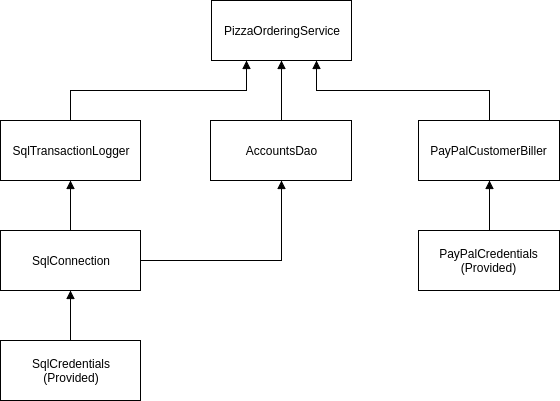
\includegraphics[width=0.7\textwidth]{renders/DependencyInjection.png}
      \caption{Dependency Graph built by Guice}
      \label{fig:depGraph}
\end{figure}

This leads to extremely simple code for the \java{PizzaOrderingService} in which the logic is entirely separated from the dependency management.

\lstinputlisting[
  caption={Pizza Ordering Service using Dependency Injection},
  label={lst:DI},
  style=javaStyle
  ]{code/technologies/DI.java}

Aside from abstracting away the dependency instantiation, dependency injection also has the added benefit in that all of a classes dependencies become part of the classes signature. There are no required dependencies that are buried within the implementation logic. This makes the code much simpler to test. The \java{PayPalCustomerBiller} used by the class is essentially hardwired into the code that does not use dependency injection (\refcode{lst:noDI}), meaning there is no way to test this class without actually billing a (fake) customer. However as the \java{PayPalCustomerBiller} used by the dependency injected code (\refcode{lst:DI}), a mock of this object (which skips the actual billing, but returns results as if it actually billed a customer) can be provided to the class and used for testing purposes.   

\subsection{Immutables - Immutability for Java}
Immutability is a programming paradigm in which once an object is created, it may never been changed. At first glance this sounds like a bad idea which will result in redundant object creation, but the positives strongly outweigh the negatives. The primary benefit of immutability is that the programmer is \textbf{guaranteed} that any object they hold a reference to, will never be changed. This concept is closely tied to the concept of writing \textit{pure} functions. These are functions which have no external side effects. That is, they take in arguments and return a value, but do not change the input arguments (or any other state contained in the program) in any way. 

These benefits are best highlighted through sample code. Consider the case of a simple website where each login attempt by a user should be logged to a database table in order to detect a hacker trying to crack a password by repeatedly trying to login as a user. For obvious reasons, this table should not store the user's password (in case of real login attempts), so this should be stripped before logging it to the database. An example \java{LoginRequest} is shown in \refcode{lst:loginRequest}. A \java{LoginAttemptLogger} class is written to handle logging these attempts to the database and is shown in \refcode{lst:loginAttemptLogger}. The \java{logLoginAttempt} method handles stripping the password from the \java{LoginRequest} and writing it to the database. 

\lstinputlisting[
  caption={An Example LoginRequest},
  label={lst:loginRequest},
  style=javaStyle
  ]{code/technologies/immutability/LoginRequest.java}

\lstinputlisting[
  caption={An Example LoginAttemptLogger Implementation},
  label={lst:loginAttemptLogger},
  style=javaStyle
  ]{code/technologies/immutability/LoginAttemptLogger.java}

However this style of code is a recipie for disaster. The \java{LoginRequest} is mutable and the \java{logLoginAttempt} method contains a side effect in that it sets the password of the \java{LoginRequest} to an empty string. Some perfectly reasonable client code is shown in \refcode{lst:clientLoginCode} in which the client logs the login request to the database and subsequently tries to log in. In this case, no user will ever be able to login as all of the passwords of the login requests are always mutated to be an empty string. Thus, having \java{LoginRequest} as a mutable object causes a critical bug that will not be caught until runtime.

\lstinputlisting[
  caption={Perfectly Reasonable Client Login Code},
  label={lst:clientLoginCode},
  style=javaStyle
  ]{code/technologies/immutability/ClientLogin.java}

The solution to this problem is to create a new \java{LoginRequest} without the user's password and log that to the database. This can be done inside of the client login code (defensive copying) before passing the \java{LoginReuqest} to the \java{logLoginAttempt}. However if mutators are provided, it is extremelty likely that they will be used somewhere in the code. Thus the best solution is simply to not provide them at all - make the object entirely immutable. This in turn requires some clunky code inside of the client login method (see \refcode{lst:clunkyImmutableClient}), but avoid the issue caused by the side effect of \java{logLoginAttempt}. 

\lstinputlisting[
  caption={Logically Correct Login Code with Extra Boilerplate},
  label={lst:clunkyImmutableClient},
  style=javaStyle
  ]{code/technologies/immutability/ImmutableClientLogin.java}

The Immutables \cite{immutablesJava} provides a framework for autogenerating fully immutable object implementations in Java. These implementations provide extremely useful functionality such as implementing builders and providing methods for updating the fields of an object in an immutable way. The immutable data structure is defined using an interface (annotated with \java{@Value.Immutable}) which contains the getter methods for each desired field of the object. A class which implements this interface in an immutable way is then auto generated by the framework and can is then used in place of the interface. An example of the interface used for \java{LoginRequest} is shown in \refcode{lst:immutableLibLoginRequest}.

\lstinputlisting[
  caption={Interface Used to Define LoginRequest using Immutables Framework},
  label={lst:immutableLibLoginRequest},
  style=javaStyle
  ]{code/technologies/immutability/ImmutableLibLoginRequest.java}

The implementation of this interface generated by the framework then provides a \java{withFieldName} method for each of the fields defined, allowing a new instance of the object with the updated fields to be obtained with a single method call as shown in \refcode{lst:loginAttemptLoggerWithImmutable}. This solves the problem of mutating the \java{LoginRequest} that the client holds a reference to and drastically simplifies working with immutable objects in Java. This framework is used exstensively at HubSpot and is a major contributor to the simplicity of writing code without bugs at the company.

\lstinputlisting[
  caption={The LoginAttemptLogger Method using the Immutables Framework},
  label={lst:loginAttemptLoggerWithImmutable},
  style=javaStyle
  ]{code/technologies/immutability/LoginAttemptLoggerImmutable.java}


\subsection{Kafka - Streaming Platform}
Kafka \cite{kafka} is a horiztonally scalable, fault tolerant, distributed streaming platform used to read and write streams of data in real time. It is an extremely high performance system and is used exstensively by the \team{} team as the primary data pipeline. Kafka runs on it's own cluster and stores streams of records inside categories known as Kafka \textit{topics}. Kafka provides two key APIs that are used at HubSpot - one for producing records to a given Kafka topic and one for consuming records from a specific Kafka topic. Kafka is used exstensively inside of the team's internal pipeline, but also as an interface between teams. For example, the teams responsible for building out and rendering the full HTML body of an email to be sent on behalf of a customer can produce this ready to be sent email to a specific kafka topic. Kafka consumers owned by the \team{} team are subscribed to this topic and thus pick up the records published to these topics and can perform the send of the email. This entirely decouples the work done by teams by simply requiring teams to put messages onto Kafka to be handled elsewhere. An obvious alternative to using Kafka would be to simply expose a REST endpoint in which the message is posted to. However simple HTTP would struggle to support the volume of requests (upwards of 25M emails per day) seen by the \team{} team. As mentioned, Kafka is horizontally scalable, meaning the number of nodes on the Kafka cluster can simply grow as the number of messages published to Kafka increases. Similarly on the consumer side, the number of deployed workers subscribed to a given topic can simply be increased in order to meet the increased number of records published to the topic.

Kafka also provides another layer of granularity - partitions. Each Kafka topic is segmented into a number of partitions. Each partition is (at any given time) owned by exactly one Kafka consumer, but each Kafka consumer may own multiple partitions. This leads to an interesting case when choosing the number of partitions to use for a given topic. Ideally, the number of partitions should be a highly composite number \cite {highlyCompositeNumbers}. These are numbers which are divisible by many other numbers, for example 24 which is divisible by 2, 3, 4, 6, 8 and 12. To illustrate why, consider the case where 9 partitions are used - the work load is only equally distributed if 1, 3 or 9 consumers are used. Thus if 3 consumers isn't enough, scaling to five consumers means four consumers will be consuming from two partitions and one will only be consuming from one partition. Using a highly composite number of partitions allows for more flexibility when choosing the number of consumers. Kafka can also handle rebalancing the workload, by redistributing the partitions when the number of consumers changes. 

When messages are produced to a Kafka topic, a decision must be made on which paritition to assign the message to. This can be done intelligently with load balancing in mind, or simply using a round robin. Partitions can also be replicated in order to provide fault tolerance.

An example of a Kafka topic with two consumers is shown in \reffig{fig:kafka}. 

\begin{figure}[H]
      \centering
      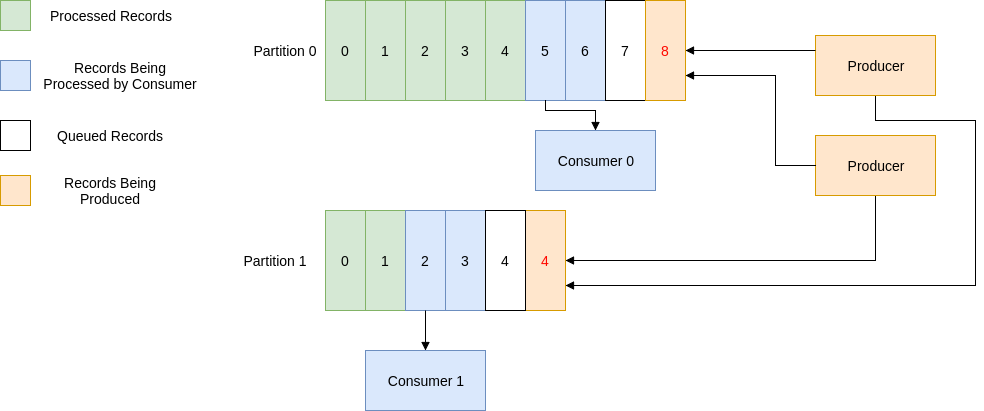
\includegraphics[width=\textwidth]{renders/Kafka.png}
      \caption{Kafka Producers and Consumers}
      \label{fig:kafka}
\end{figure}  

The current situation is outlined as follows:
\begin{itemize}
\item{Consumer 0 has successfully processed (and commited) messages 0 to 4 and is currently processing messages 5 and 6}
\item{Consumer 1 has successfully processed (and commited) messages 0 and 1 and is currently processing messages 2 and 3}
\item{Message 7 in partition 0 and message 4 in partition 1 have both been successfully produced and commited to the log}
\item{Message 8 in partition 1 and message 4 in parition two will be the next messages produced by the producers.}
\end{itemize}

Each message published to a Kafka partition gets an incremental id known as an \textit{offset}. Consumers are responsible for managing their offset in the message stream. Thus consumers can be configured to start from any offset, which can even allow for reprocessing of data should the need arise. This has been useful in the past at HubSpot when a bug has caused emails to fail to send. The consumers can have their offsets reset to when the bug first surfaced and the emails will be resent. However this is a delicate process and is only used as a last resort. The offsets for consumers 1 and 2 in \reffig{fig:kafka} would be 4 and 1 respectively.

An key concept to understand about Kafka is that consumers are presented with batches of records, of a configurable size. The batch size in \reffig{fig:kafka} is two. The records inside the batch may be processed out of order, but the batch of records is considered completed \textbf{only when every record in the batch has been processed}. In Kafka, only an entire batch of messages can be marked as processed. For example consider consumer 0 in \reffig{fig:kafka}. Should the consumer succeed to process message two, but fail to process message three, Kafka must be notified of the failure to process the batch of messages (or will notice a timeout) and the entire batch will be retried.


Another interesting concept in Kafka is consumer groups. Consider the case where two entirely separate sets of workers (running different code) need to read from the same Kafka topic. Both sets of workers should be able to process every message that is published to the Kafka and this is what consumer groups provides. Without consumer groups, another worker could be set up in order to read from the Kafka topic, but as discussed, it would only acquire a certain number of partitions and thus miss some messages (and steal messages from existing workers). The solution is to specify the consumer group that each running worker belongs to. In this case, since there are two sets of workers, both doing different things, there should be two consumer groups. Kafka will then treat all of the consumers in each consumer group as if there are no other sets of workers reading from the Kafka topic. This feature is best understood by considering the two edge cases:

\begin{itemize}
\item{If all workers are in the \textit{same} consumer group, Kafka simply load balances the partitions across the number of workers}
\item{If all workers are in \textit{different} consumer groups, each worker will have its own offset in \textbf{all} of the partitions. That is, the worker responsible for partition zero in consumer group A may have a current offset of 100, while the worker responsible for partition zero in consumer group B may have a current offset of 0. This is essentially, publish-subscribe (pub-sub) behaviour. All of the workers will simply see all of the events and the rate of consumption of a certain worker has no impact on the rate of consumption of another worker.}
\end{itemize}

Continuing with the previous example (of having all of the emails to be sent through HubSpot contained on a Kafka topic), the following consumer groups could be set up in order to both send every email that appears on the topic and to bill each customer for each email that appears on the topic. This is also shown in \reffig{fig:consumerGroups}
\begin{labeling}{SENDING}
\item[SENDING]{This consumer group would contain all of the \team{} team's consumers. There would likely be a lot of consumer's in this consumer group in order to keep up with the time consuming process of actually sending the emails on behalf of the customers. These would be time critical and thus performance and efficiency would be critical. The delta between the current offset (the index of the most recently produced message) and the oldest offset (the index of the oldest message still being processed) for each partition would likely be carefully monitored to ensure the consumers are not falling behind}
\item[BILLING]{This consumer group would perhaps simply read the account number of the customer sending the email and bill that customer. This consumer group would be considerably less time critical and would likely only need to perform some light weight task for each message on the Kafka topic.}
\end{labeling}


\begin{figure}[H]
      \centering
      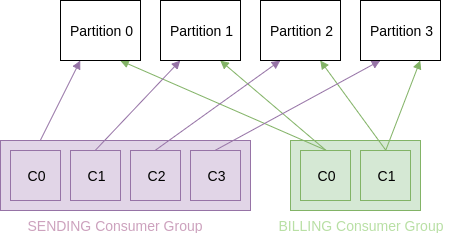
\includegraphics[width=0.6\textwidth]{renders/ConsumerGroups.png}
      \caption{Partition Assignments with Multiple Consumer Groups}
      \label{fig:consumerGroups}
\end{figure}  

A final note of interest regarding Kafka is that it provides and \textit{at-least-once} guarantee that messages will arive at consumers for processing. If a single message in a batch of messages cannot be processed for whatever reason, the entire batch will be retried. Thus external idempotency logic is required in order to obtain an \textit{exactly-once} processing guarantee. The \team{} team uses a simple HBase table in order to lock each email that is to be sent, prior to actually sending it. 

% \subsection{MySql}
% Indexes, liquibase, InnoDB

% \subsection{HBase}

% \subsection{ZooKeeper (Circus)}\

% \subsection{Maven - Dependency Management}

\subsection{Hadoop}

\subsection{gRPC and Protobuf}



\section{Email Specific Technologies}
\subsection{DNS} \label{sec:DNS}
Although not entirely email specific, DNS is extremely critical for the \team{} team. Aside from teams working on the HubSpot platform, most other teams need not concern themselves with DNS at all. 

DIAGRAM OF RECORDS?
DKIM SELECTORS **
each of the record types, when an email arrives what is looked at, look at the tld, then zones on that tld then record types and key values etc. UDP typically, fallback to TCP
\subsection{SMTP} \label{sec:smtp}

\section{System Management and Health Monitoring}
While working on projects of this magnitude, bugs and issues are an inevitability. The amount of traffic seen by these systems compounds any small issues or bugs present in the system. As such, it is critcal to have systems in place which monitor the health of the system and inform the team of any potential issues with the system. Whatsmore, these issues must be continuously examined and remedial action must be taken where applicable. The \team{} team made use of several tools and methods for monitoring the health of their systems, a subset of which are outlined below:

\subsection{Log4j2}
Log4j2 \cite{log4j2} is a Java framework which is provides facilities for logging to different log levels and advanced log filtering (for example with regular expressions). This provides an excellent facility for understanding why systems are behaving unexpectedly in production. A common pattern is to insert log messages to a low priority log level (eg DEBUG) which describe the state of the system or the code path taken. Typically when the system is behaving normally, a highger priortiy log level is set (eg INFO) meaning these finer grained log messages are skipped. However, should an issue arise, the log level can then be easily switched to the lower priority temporarily to get a more detailed insight into why the system is misbehaving. This pattern allows detailed log messages to be produced only when they are needed, reducing the amount of noise present in the logs. The framework also provides the ERROR debug mode which can log error messages as uncaught exceptions without killing the currently executing thread.

\subsection{Sentry}
Sentry \cite{sentry} is an online platform which logs uncaught exceptions that arise during program execution. This greatly simplifies the task of finding out the reason for a system fault or failure without the need to trawl through pages of log files. Sentry logs the full stack trace associated with an exception, the time of occuence and other pieces of meta data such as the name of the deployable. It uses this data to monitor the occurences of particular exceptions over time, provides facilities for opening and closing GitHub issues and most importantly, to send an email to all those subscribed to the project (eg the \team{} in this case) when an exception occurs. Sentry proves to be extremely useful at deploy time. Obviously when deploying new code to production servers, one must be sure that the changes did not cause the system to enter an unhealthy state. Provided the code is well written and that unexpected exceptions that occur are not silently swallowed, Sentry can be monitored at deploy time in order to help provide the engineer with confidence that the deployed changes were non breaking. Sentry also provides support for integrating into the aforementioned Log4j2. Sentry can monitor ERROR level log messages that are produced by Log4j2 and subsequently log these error messages to sentry. As an engineer this combination of tools is extremely useful for indicating that the system has found an issue, without killing the thread. This is ideal in cases where some work has been done and the system has encountered a critical error, but does not need to be restarted. This mitigates the need to repeat the work, but still enforms the team that an error has occured by logging an exception to Sentry.

\subsection{SignalFX}
SignalFX \cite{sigfx} is a online tool for recording metrics and data visualization. Gathering and analysing metrics is a key part of ensuring the health of a comlpex system. When things start to fail, SignalFX is the first place engineers look to. SignalFX essentially allows data to be dumped to the cloud and for complex graphs and charts to be rendered in real time using this data. SignalFX supports creating dashboards consiting of many of these graphs and charts. The \team{} team has several of these dashboards, each encapsulating a single part of the system. When problems inevitably arise, the team can examine these dashboards in order to try and isolate and find the problem. Once remedial action has been taken, the dashboards can be monitored to ensure the desired effect takes place. Being able to see these metrics in close to real time is incredibily useful for diagnosing faults with the system. It also serves as an excellent mechanism for finding parts of the system that can be improved. For example, critical code paths can be timed and the results logged to sentry. This allows accurate inferences to be made about parts of the system and allows the team to target these parts.

SignalFX also allows for detectors to be configured. For example, a chart could be created monitoring the number of emails sent in the past minute by each IP address responsible for sending emails. A detector can then be put in place to detect if this number falls below a certain threshold. Detectors can be configured to alert via email and slack when they fire, allowing engineers to be notified. 

SignalFX also supports complex data aggregations. This is beneficial as it decouples calculations that need to be done on metrics from the code which the metrics are monitoring. Perform any sort of data manipulation in performance critical code paths is obviously not desirable when every millisecond counts. Instead, metrics gathering is as simple as producing the data to SignalFX. The complex graphs and charts can then be configured inside of the SignalFX tool, entirely independant to the production code. 
\chapter{Tasks Undertaken}
Throughout the course of the internship, a variety of tasks were undertaken and completed.  
For the sake of brevity a small subset of the most interesting of these tasks are outlined below. 

\section{Rebuilt DNS Management System}
DNS plays an important part in sending emails. As discussed in \refsec{sec:DNS}, there a several DNS records that must be maintained for a server to send email. As HubSpot aims to offer as seemless an experience as possible to it's customers, it attempts to take care of as much of the DNS settings as possible on behalf of the customer. Ultimately however, if a customer want's HubSpot to send their marketing emails through an SMTP domain of \java{emails.company.com}, these DNS records must be obtainable at that domain as discussed in \refsec{sec:DNS}. 

As things change at HubSpot, it is quite likely that these DNS records would need to change over time. For example, if the customer should add another dedicated IP address to their account, this would have to be added to their SPF record. At first glance this would require HubSpot's customers to be frequently changing their DNS records, something most customer's would not be overly comfortable with. The solution to this problem, as with so many problems in computer science, is indirection. 

The Domain Name System supports the concept of including other DNS records, even from entirely different domains. This is exactly the behavior that lets HubSpot manage their customers' DNS on their behalf. For example, instead of \java{emails.company.com} having the SPF record which contains their allowed sending IPs and having to change it should their sending IPs change, they can simply setup this record as a pointer to another DNS record, a record on HubSpot's domain. Clients who require the SPF record for for \java{emails.company.com} will be informed to use the record contained on HubSpot's domain instead. An example of this is shown in \reffig{fig:dnsIncludes}, where 99 is the customer's HubSpot identification number. A similar setup exists for customers' DKIM records.

Thus the customer only ever needs to set up the DNS pointers to HubSpot's domain once. Once that is done, HubSpot can control the actual values of those DNS records on behalf of the customer. 

\begin{figure}[H]
      \centering
      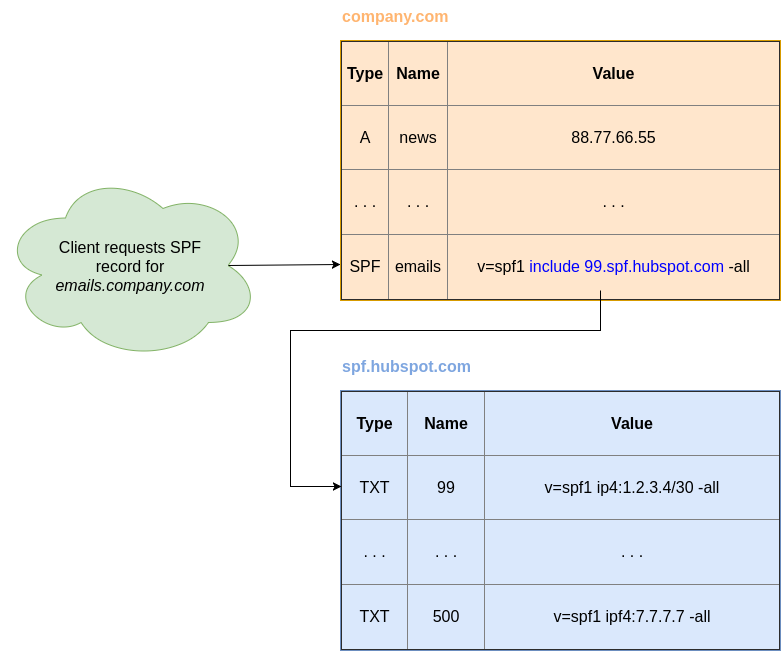
\includegraphics[width=0.8\textwidth]{renders/DnsIncludes.png}
      \caption{DNS Includes for \textit{emails.company.com}, HubSpot Customer 99.}
      \label{fig:dnsIncludes}
\end{figure}

Initially, all of the DNS records living on the \java{spf.hubspot.com} (the ones which customers include) were created at various points in the code. There was no definition for exactly what DNS records should be available and where they should be available for a given account. Some of the DNS record creation was coupled to the code that was responsible for creating new customer accounts, but as time went on, different DNS records were required, resulting in redundant DNS records being created. There were also several scheduled Cron jobs, jobs which run periodically, responsible for checking the current status of the DNS records and attempting to adjust them as necessary. There were no unit tests for any of the code which synced DNS records. Some of these jobs concluded that different values should exist for the same DNS record, resulting in the jobs competing with each other and updating DNS records every time they ran. It was also unclear what DNS changes were required if accounts were updated. This led to the creation of an entirely new DNS management system.


\subsection{Requirements for the Management System}
Prior to beginning to rebuild the system, an analysis of the current system was required to ensure all of the required functionality contained in the old system would be included in the new system. Another important step was to consider what the \textit{ideal} system would look like. There were two main options to consider:

\begin{enumerate}
    \item{Create all of the DNS records required when the corresponding customer account was created. As discussed previously, it is likely that the value of these DNS records would change over time. Thus, this would also require periodic CRON jobs in order to compare the current state of a customer's DNS records against what the system believes their DNS records should be and to update them accordingly. The downside to this approach was having the required DNS records defined and maintained in two separate places - once during account creation and once during the DNS record synchronization.}
    \item{Abstract away all DNS record creation from the account creation process and write the periodic CRON jobs in such a way that they can also create brand new DNS records as necessary. The downside of this approach is that there would be a period of time in which the accounts would be created, but have invalid DNS records, which could be problematic if not managed appropriately.}  
\end{enumerate}

After some consideration, it became clear that option two was the better choice. The period of time in which the accounts would be created but have invalid DNS records could be managed rather simply. Provided the jobs were written correctly, this approach would have the benefit that it could sync DNS records for arbitrarily complex entities. For example, initially the customer's account was all that was required in order to keep their DNS records in sync. However as time went on, other types of DNS records also needed to be maintained, which could not necessarily be deterministically generated from just a customer's account. An example of this is IP addresses which are owned by HubSpot, but not yet in use by any customer. These IP addresses should have specific DNS records in place. However by definition, these IP addresses are not yet assigned to any accounts. Thus the new system should also be able to sync DNS records based on IP addresses. In the past the solution to this problem would have been to simply create yet another periodic CRON job to maintain those DNS records, making it even more difficult for an engineer to know where in the code a given DNS record is maintained.

Another important concept are DNS \textit{zones} (sub domains). For easier organization and management of a large number of DNS records, a top level domain (TLD) can be further sub-categorized into zones. In the previous example domain \java{emails.company.com}, the TLD is \java{company.com} and a zone on that TLD is \java{emails}. The purpose of DNS zones is to allow finer grained control for a domain with a large number of DNS records. For example, a customer could setup all of the records required for HubSpot's email marketing on a single zone, the \java{emails} zone, isolated from all of the domain's other records (e.g. for their website, internal email etc). 

The requirements of the new system were determined to be the following:
\begin{enumerate}
      \item{It can sync DNS records for arbitrary entities (Accounts, IP Addresses etc)}
      \item{The code for generating the values of specific DNS records should be decoupled from the code which actually runs the job. This allows for comprehensive unit testing of the code which generates the records.}
      \item{It should only make external requests to update records which are no longer valid.}
      \item{It should group the records required for a given entity by zone, allowing for easier record lookups and updates}
\end{enumerate}

\subsection{Implementation of the System}
The first task was to decide how the code which builds the DNS records should be organized. It was imperative to have this code be as clear and concise as possible. The DNS records themselves are hosted on various providers (e.g. Cloudfare), but the Platform team in HubSpot provides a simple client for working with these records (creating records etc). A \java{DnsRecordBuilder<T>} interface was defined and is shown in \refapp{appendix:dnsManagement} \refcode{lst:dnsRecordBuilder}. This interface defines the following methods:

\begin{itemize}

      \item{\java{Multimap<String, RecordRequest> buildSpfRecords(T entity)}}
      \begin{itemize}
            \item{This method will generate the SPF record required for a given entity of type \java{T} (e.g. an account)}
            \item{Equivalent methods are also defined for MX, A and DKIM records}
            \item{The \java{RecordRequest} object is a Java object which contains can be passed to the DnsClient library to create / update / delete the given record}
            \item{These methods return Multimaps (which is essentially a \java{Map<String, Collection<RecordRequest>>}) which use the record's zone as the key}
            \item{All of these methods are defaulted to returning empty multimaps (if they are not overridden)}
      \end{itemize}

      \item{\java{boolean appliesTo(T entity)}}
      \begin{itemize}
            \item{This method specifies whether or not this particular implementation of \java{DnsRecordBuilder} should apply to this entity}
            \item{For example if the entity was an account, this method can be used to specify that only accounts with dedicated IP addresses should use this \java{DnsRecordBuilder}}
      \end{itemize}

      \item{\java{Map<String,DnsConfiguration> getDnsConfigByZone(T entity)}}
      \begin{itemize}
            \item{The \java{DnsConfiguration} is a Java object which contains a zone name and a list of \java{RecordRequest} objects (which contains all of the records to be created)}
            \item{This method has a useful default implementation which aggregates all of the multimaps returned by each methods that builds the records of each type (SPF, DKIM, A, MX) into a single multimap. The returned map of DNS configurations by zone can then be built and returned.}
            \item{This is the most common method called on this interface as it invokes all of the other methods, returning the exact DNS configurations (by zone) needed to keep the given entity up to date.}
      \end{itemize}

      \item{\java{Map<String, String> buildPtrRecords(T entity)}}
      \begin{itemize}
            \item{The final method defines the PTR records that should be created for this entity, returning a map containing the IP address as the key and the host name corresponding to this IP address as the value}
            \item{As discussed in \refsec{sec:DNS}, PTR records are used to perform reverse A lookups, defining the host name associated with an IP address.}
      \end{itemize}
\end{itemize}

Implementations of this interface can then be created for a given entity type. For example, a \java{DefaultAccountDnsRecordBuilder<Account>} was created to encapsulate all of the records that need to be created for every HubSpot customer account. Similarly, a \java{UnassignedIpDnsRecordBuilder<IpAddress>} was also created to encapsulate all of the DNS records required for an unassigned IP address. The \java{IpAddress} object contains the status of the IP address (whether its associated with a customer account or not etc). The \java{appliesTo} method of this implementation can then check this field and only return DNS records if the \java{IpAddress} is in fact unassigned. As time went on, more of these \java{DnsRecordBuilder} implementations were created, encapsulating different DNS requirements. This provides a very clean and extensible way of defining DNS records which are deterministically built from arbitrary entities.

The next step in the implementation was to write an intermediate class which given an entity of type \java{T}, applies all of the \java{DnsRecordBuilder}s corresponding to the entity and finds out which records need updating. 

A \java{Map<Class, List<DnsRecordBuilder>>} is created and is used to determine the list of \java{DnsRecordBuilder}s that need to be applied to a given entity by simply looking up the entity's class in the map. The \java{getDnsConfigurationsByZone} method defined above is invoked on each of the builders in the list, generating all of the DNS records that need to be present for the given entity. 

Finally another piece of logic was written to determine which records need to be updated for the entity. This is done by checking the records against an in-memory cache, a database cache and finally live DNS. This reduces the number of real DNS queries that need to be made. The in-memory cache and database cache would be frequently invalidated to ensure cached DNS records had not become stale. Any records which require updates are then added to a \java{List<DnsConfiguration>} and returned to the caller to perform the actual updating. This code segment is provided in \refapp{appendix:dnsManagement} \refcode{lst:recordBuilderApplier}.

The final step was to create the Cron job which will use the above code to keep the required DNS records in sync. The HubSpot development platform provides a simple means of registering jobs which are to be run on a schedule. The benefits of the extra complexity of the above code are seen in the implementation of the job. The job simply fetches all of the entities of interest (accounts, IP addresses etc) from a database. For each of these entities, the job calls the method from the intermediate class as discussed in the previous paragraph using the entity as a parameter. This method returns the list of records which need be updated or created. The job then handles performing the required DNS updates. A simplified version of the job in which the DNS records for all accounts are synced is shown in \refapp{appendix:dnsManagement} \refcode{lst:dnsSyncJob}.

\break
\section{CIDR Minimization Algorithm}
As discussed in \refsec{sec:DNS}, SPF records are a vital part of authorization when it comes to sending emails. SPF records are typically used to specify a set of IP addresses that a particular domain may send emails from. An important aspect of SPF records (or more specifically, the underlying TXT record) is that the length of the entire record value (which is a simple string) should be at most 255 characters as per RFC 7208 \cite{spfRFC}. Given the fact that a particular HubSpot customer may potentially send email over any one of tens of HubSpot owned IPs, this can cause problems. 

One of the upgrades customers can avail of is purchasing dedicated IP addresses, which will be used for their email traffic and theirs only. This allows the customer to build up a good IP reputation without the risk of the reputation being harmed by other HubSpot customers who may send lower quality email. HubSpot owns a large number of IP addresses in order to facilitate this. One of the other tasks undertaken during the course of the internship was automating the process of setting up email sending accounts for new dedicated customers. Prior to this automation, one of the decisions that needed to be made by support staff working with customers was which IP address(es) to assign to customers. Some customers have existing IP addresses and IPs should be selected in order to minimize the length of the resulting SPF record that the customer will have. SPF records support CIDR notation (see \refsec{sec:CIDR}) of IP addresses, meaning smart IP selection can save valuable characters in a customer's SPF record. Thus an important step in automating the setting up of customer accounts with dedicated IP addresses was automating the IP address selection, while still minimizing the resulting SPF records.

\subsection{CIDR Notation} \label{sec:CIDR}
CIDR (Classless Inter-Domain Routing) notation is a compact way to represent an IP address along with its associated subnet mask and network prefix \cite{cidr}. With regards to SPF records, it is useful as it can be used to compactly represent a set of IP addresses. This set consists of the IP addresses of all of the hosts on the sub-network (subnet) specified by the network prefix. This section will primarily discuss CIDR notation for version four (IPv4) IP addresses, though all of the same logic holds for version six (IPv6) IP addresses. 

Typically IP addresses are represented as quartet of period separated integers ranging from 0 - 255, for example, $192.168.1.1$. However, this representation is simply employed in order to make reading IP addresses easier for humans. In actuality, version four IP addresses are more simply represented as 32 bit integers. Each of the numbers in the quartet can take on one of 256 values. Thus

\begin{equation}
\begin{split}
\log_2 256 = 8\,bits\,per\,element\,in\,quartet \\
8\,bits\,per\,element \times 4\,elements\,in\,quartet = 32\, bits
\end{split}
\end{equation}



$192.168.1.1$ could be represented as a 32 bit integer by using $192$ as the most upper (most significant) 8 bits, $168$ as the next 8 bits and so on. CIDR notation contains the IP address in question, followed by a slash and a number, for example $192.168.1.2/31$. CIDR notation partitions the 32 bit representation of the IP address into two pieces - the upper bits make up the network prefix and the remaining bits are used to specify the specific host on that network. The number following the slash denotes the number of bits to use for the network prefix. Thus $192.168.1.3/31$ specifies that 31 out of the 32 bits should be used for the network prefix and all other bits should be zeroed in order to obtain the network address. This implies that the network address is $192.168.1.2$. This is because the least significant byte of this IP address is 3, or $(0000\enspace0011)_2$ in binary, and the last bit is to be zeroed meaning the last byte of the network address becomes $(0000\enspace0010)_2$, which is 2 in base-10. 

CIDR notation can thus be used to represent a set of IP addresses, provided they are contiguous. The set has a cardinality that is an integral power of 2 and the first IP address in the set lies on a CIDR boundary. The set of IPs $\{192.168.1.0, 192.168.1.1\}$ can be represented using CIDR notation as $192.168.1.0/31$. The logic here is that the address of the subnet containing the hosts of interest is provided and the implied set of IPs is the set of all IP addresses of the hosts on that subnet.  Thus if a customer owns these two IP addresses, their SPF record can simply contain the CIDR notation value of the subnet which contains the two IP addresses, reducing the number of characters required by almost half. This is due to the fact that $/31$ implies that there is one bit (the last bit) which identifies the host on the subnetwork defined by $192.168.1.0$. This bit can either be a zero or a one, yielding the two possible IP addresses that were started with - $192.168.1.0$ or $192.168.1.1$.

\subsection{A Simplified Version of the Algorithm}
The main objective of the algorithm is summarized as follows (Note if the CIDR post fix is omitted, $/32$ is implied): \hfill\break\break
Given a set of existing IP addresses $S_e$ (the \textit{existing} set) and a set of available IP addresses $S_a$ (the \textit{available} set), choose a set of $n$ IP addresses $S_c$ (the \textit{chosen} set) from $S_a$ such that the resulting number of characters in the CIDR representation of $S_f$ (the \textit{final} set) is minimized, where 

\begin{equation}
S_f = S_e \cup S_c
\end{equation}

An example scenario in which the algorithm could be used is given in \refeq{eq:ipAlgExample}
\begin{equation}\label{eq:ipAlgExample}
\begin{split}
 &   S_e = \{1.1.1.1,\enspace1.1.1.2\} \\
 &   S_a = \{1.1.1.0,\enspace1.1.1.3,\enspace1.1.1.4,\enspace1.1.1.5\} \\
 &   n = 2 \\
\end{split}
\end{equation}

In this scenario, the algorithm should result in $S_c = \{1.1.1.0,\enspace1.1.1.3\}$, resulting in $S_f = \{1.1.1.0,\enspace1.1.1.1,\enspace1.1.1.2,\enspace1.1.1.3\}$ which is represented in CIDR notation as $S_f = \{1.1.1.0/30\}$. Critically, although the set of IPs $\{1.1.1.1,\enspace1.1.1.2,\enspace1.1.1.3,\enspace1.1.1.4\}$ are contiguous, the CIDR representation of these IPs is $\{1.1.1.1,\enspace1.1.1.2/31,\enspace1.1.1.4\}$ \textbf{not} $\{1.1.1.1/30\}$ as first IP does not lie on a CIDR boundary.

Although the algorithm could likely be brute forced by generating every possible set of IP addresses and choosing the one with the fewest characters in the CIDR representation, this algorithm would run in exponential time making it less than ideal.

In order to attempt to gain some deeper insight into the problem, a common mathematical approach was used in which a simpler version of the problem was considered - the case where there is no existing IPs ($S_e = \{\}$). For convenience, a new variable $t$ is also introduced to represent the total number of IPs in the final set (the cardinality of $S_f$). Thus:

\begin{equation}
t = |S_f| = |S_e| + n
\end{equation}

The first step of the algorithm requires determining the largest possible CIDR block that could be obtained for a given $t$. The number of IPs in a CIDR block is related to the number of bits available for representing the hosts on the subnetwork. Thus, the number of IPs in a CIDR block must always be an integral power of 2. This is shown in \reftbl{tbl:cidrBlockSize}. 

The calculation for the number of host bits $n\sub{hb}$ is shown in \refeq{eq:numHostBits} where $n\sub{ab}$ is the number of address bits (the value after the $/$ in the CIDR address)

\begin{equation}\label{eq:numHostBits}
n\sub{hb} = 32 - n\sub{ab} 
\end{equation} 

The calculation for the number of hosts on the subnetwork ($n\sub{hosts}$) is given by the number of digits that the number of host bits $n\sub{hb}$ can represent and is shown in \refeq{eq:numHosts}.

\begin{equation}\label{eq:numHosts}
n\sub{hosts} = 2 ^ {n_{hb}}
\end{equation}

\begin{table}[H]
\caption{The Size of CIDR blocks as a function of $n_{hb}$}
\label{tbl:cidrBlockSize}
\centering
\begin{tabular}{l l l}
\toprule
\textbf{Example Address} & \textbf{Number of Host Bits $n\sub{hb}$} &\textbf{Number of IPs in Block $n\sub{hosts}$} \\
\midrule
1.1.1.0/32 & 0 & 1\\
1.1.1.0/31 & 1 & 2\\
1.1.1.0/30 & 2 & 4\\
1.1.1.0/29 & 3 & 8\\
... & ... & ...\\
1.1.1.0/1 & 31 & $2 ^ {31}$\\
\bottomrule\\
\end{tabular}
\end{table}

Thus, the largest possible block of CIDR IPs for a given $t$ can be obtained by finding the highest integral power of two that is less than or equal to $t$. For example, if $t = 10$, then 8 would be the largest possible CIDR block as $2^3 = 8$ but $2^4 = 16$.

An importance concept of the algorithm is assigning each IP address to a certain bucket. This assignment process needs to know what bucket size to use. Critically, the bucket sized used will be an integral power of 2 aligning with the above table. The IPs will be placed into the bucket that represents the subnet that they would be contained within for a given number of host bits. Logically, the presence of a filled bucket indicates that a CIDR block can be formed from the set of IPs contained in that bucket. An example is shown in \reffig{fig:exampleIpsByBucket4}. In this case, bucket $1.1.1.0$ is full as the bucket size is 4, meaning the IPs inside it can be used to create a CIDR block of size 4 - $1.1.1.0/30$.

\begin{figure}[H]
      \centering
      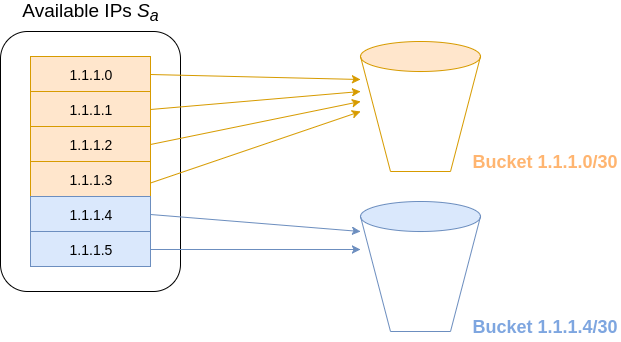
\includegraphics[width=0.8\textwidth]{renders/IpsByBucketSize4.png}
      \caption{Assigning IPs to Buckets with a Bucket Size of 4}
      \label{fig:exampleIpsByBucket4}
\end{figure}

As discussed, the bucket size will be an integral power of 2, but an important question is which integral power of 2. The algorithm starts by assigning the IPs to their buckets using a bucket size equal to the largest possible CIDR block that can be obtained for the given $t$. As discussed previously, this is the largest integral power of 2 that is less than or equal to $t$.

At this point, the algorithm begins to take shape. Consider the situation represented in \reffig{fig:exampleIpsByBucket4} along with a value of $t = 4$. The initial bucket size will be 4 and the presence of a filled bucket ($1.1.1.0/30$) indicates that a CIDR block of the bucket size can be created. Since the bucket size is equal to the desired number of IPs, the optimal choice is the $1.1.1.0/30$ block. The algorithm can return this block and it will be the optimum set of addresses to choose, to minimize the number of characters in the SPF record.

Next consider the situation represented in \reffig{fig:exampleIpsByBucket4} along with a value of $t = 6$. The initial bucket size will still be 4 (as this is the largest integral power of 2 less than or equal to $t$). Thus, the algorithm will again detect that the $1.1.1.0/30$ bucket is full and select this block of four IPs. However the algorithm must return a total of $t = 6$ IPs and therefore must select a further 2 IPs. The algorithm accomplishes this by making a recursive call. By removing all of the (so far) selected IPs from the set of available IPs (forming $S_a'$, the \textit{available} set for the next call) and setting the new value of $t$ to be the remaining number of IPs required ($t'$ = 2), a recursive call will simply find the best set of IPs from what is left. This is shown in \reffig{fig:exampleIpsByBucket2} in which the recursive call would return $1.1.1.4/31$ as this bucket is full. The selected IPs from each recursive call are then unioned, returning the optimum set of IPs - $\{1.1.1.0/30,\enspace1.1.1.4/31\}$

\begin{figure}[H]
      \centering
      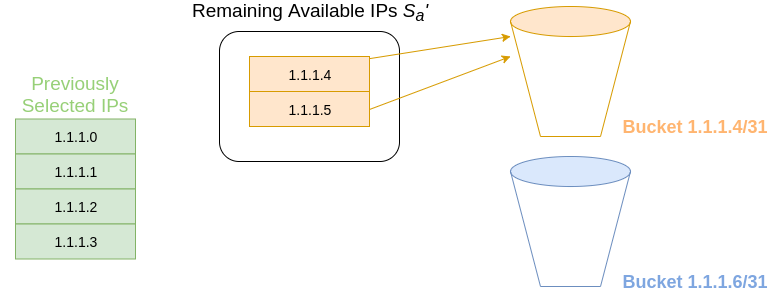
\includegraphics[width=0.8\textwidth]{renders/IpsByBucketSize2.png}
      \caption{Assigning Remaining IPs to Buckets with a Bucket Size of 2}
      \label{fig:exampleIpsByBucket2}
\end{figure}

In the case of $t = 7$, the algorithm would proceed as before, with one extra recursive call with $t = 1$. Assuming there were sufficient IPs available (the number of IPs in the diagrams were limited for brevity), the algorithm would have selected the same 6 IPs as before and the final call would be the trivial case of $t = 1$ in which a random IP can be selected. At each stage, the set of IPs returned from the recursive calls can then be unioned with the current call's chosen IPs, and the unioned set returned. 

The final possibility to consider is what should be done when no buckets are filled. In this case, the algorithm should not select any IPs at this bucket size. Instead, it should reduce the bucket size to the next highest integral power of 2 and recurse, setting $t$ equal to this reduced bucket size. However, there is another important step, the need for which is best illustrated with an example. A diagram of this situation is shown in \reffig{fig:ipAlgTrickyCodePath}

If the initial value for $t$ is 6, the initial bucket size will be 4. If no buckets of size 4 are filled, the algorithm will then recurse. Let the total number of IPs required that is used for this recursive call be denoted as $t_1'$. Thus, for the recursive call, $t_1' = 2$ (the next largest integral power of 2 as discussed previously) and the set of available IPs is unchanged $S_{a_1} = S_a$. Let the set of chosen IPs returned from this first recursive call be denoted as $S_{c_1}$.

The initial call required 6 IPs to be returned, however this first recursive call will return 2 IPs that should be used, $\{1.1.1.0,\enspace1.1.1.1\}$ in this case. Thus a second recursive call is required. Let the total number of IPs required that is used for this second recursive call be denoted as $t_2'$. $t_2'$ is calculated using the formula given in \refeq{eq:secondRecurseT2}. This is simply the remaining number of IPs that need to be chosen after the first recursive call. In this case, $t_2' = 4$. 

\begin{equation}\label{eq:secondRecurseT2}
t_2' = t - t_1'
\end{equation}

Finally, the set of available IPs that is used for the second recursive call ($S_{a_2}$) is given by \refeq{eq:availableIpsSecondRecurse}. This is the initial set of all available IPs, with the IPs chosen from the first recursive call omitted.

\begin{equation}\label{eq:availableIpsSecondRecurse}
S_{a_2} = S_a - S_{c_1}
\end{equation}

\begin{figure}[H]
      \centering
      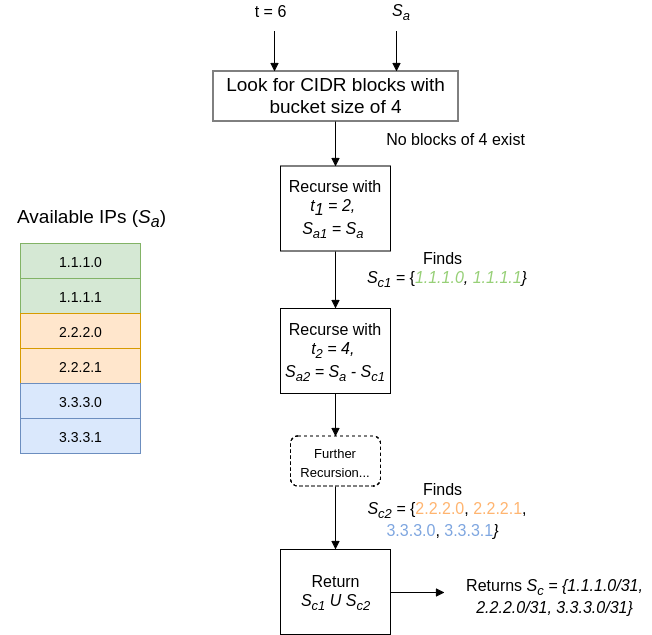
\includegraphics[width=0.8\textwidth]{renders/IpAlgTrickyCodePath.png}
      \caption{Code Path when Algorithm Does Not Find Full Bucket}
      \label{fig:ipAlgTrickyCodePath}
\end{figure}

The steps of the algorithm (for the simplified case of having no existing IPs) are shown below:
\begin{itemize}
\item{Set bucket size to be largest integral power of 2 that is less than $t$}
\item{Assign all available IPs into buckets using the calculated bucket size}
\item{If a bucket is full}
  \begin{itemize}
  \item{Add all of the IPs in the bucket to the set of chosen IPs ($S_c$)}
  \item{Remove all of the IPs in the bucket from the set of available IPs (forms $S_a'$)}
  \item{Calculate $t'$ as $t - bucketSize$}
  \item{Recurse using $S_a'$ and $t'$ (if necessary)}
  \end{itemize}
\item{Otherwise}
  \begin{itemize}
  \item{Recurse using next biggest integral power of 2 and the initial set of available IPs}
  \item{Recurse using the remaining number of IPs required and the set of available IPs, excluding those returned from the previous recursive call}
  \item{Return the union of the results of the two recursive calls.}
  \end{itemize}
\end{itemize}

\subsection{Extending the Algorithm to Support Existing IPs}
Now that a solution to the simplified problem where $S_e = \{\}$ has been formed, the more complex initial problem could now be tackled. However upon closer inspection, there is only one extra point to consider when the set of existing IPs is non empty: \textbf{the final set must be a super set of the set of existing IPs}. 

The algorithm now requires the following arguments:

\begin{itemize}
\item{A list of available IPs - $S_a$}
\item{A list of existing IPs - $S_e$}
\item{The total number of IPs desired - $t$}
\item{The bucket size to use - $b$}
\end{itemize}

The main changes to the algorithm are the following:

\begin{itemize}
  \item{Assign the existing IPs ($S_e$) to buckets using the provided bucket size}
  \item{(separately) Assign the available IPs ($S_a$) to buckets using the provided bucket size}
  \item{For each of the \textit{existing} IP buckets $S_{e_i}$}
      \begin{itemize}
      \item{Calculate $b^*_i$, the number of IPs required to fill the bucket (\refeq{eq:ipsToFillBucket})}
      \item{If the number of IPs in the corresponding \textit{available} IP bucket ($S_{a_i}$) equals $b^*_i$, the union of the two buckets creates a CIDR block and should be added to the currently chosen set of IPs ($S_c$), as long as it doesn't $|S_c|$ to become larger than the total number of desired IPs, $t$}
      \item{If the size of $S_c$ is now equal to $t$ (the total number of IPs required), $S_c$ can be returned.}
      \end{itemize}
\end{itemize}


\begin{equation}\label{eq:ipsToFillBucket}
b^*_i= b-|S_{e_i}|
\end{equation}


This shows that the only logical change is that the number of IPs required to fill the existing IP buckets should be examined, rather than searching for full buckets from the available pool. 

As with the simplified case, this method may require some recursion after the above steps. The recursive call in this case is actually simpler, but depends on the current state of the algorithm. As previously mentioned, all of the IPs in the existing set should be contained in the final set. If the algorithm reaches a state where all of the existing IPs have been used, but there is still a number of IPs to be selected, the algorithm can simply fallback to the previous case where $S_e = \{\}$. Otherwise, the algorithm recurses using the remaining available IPs, the remaining \textit{required} IPs (this is the set of existing IPs that have not yet been used), the remaining number of IPs required to be chosen and the next bucket size to use which is one less than the current bucket size.

Consider the following example as shown in \reffig{fig:ipsByBucketExisting4}.
\begin{itemize}
\item{$S_e = \{1.1.1.0, 2.2.2.0\}$}
\item{$S_a = \{1.1.1.1, 1.1.1.2, 1.1.1.3, 2.2.2.1, 2.2.2.2\}$}
\item{$t = 7$}
\end{itemize}

As $t = 7$, the initial bucket size $b$ would be 4 and the IPs would be assigned to buckets as shown in \reffig{fig:ipsByBucketExisting4}

The algorithm would then proceed in the following manner:
\begin{itemize}
\item{Examine each existing ($S_{e_i}$) and available ($S_{a_i}$) IP buckets in pairs}
\begin{itemize}
\item{Calculate $b_i^*$ for $1.1.1.0/30$ as per \refeq{eq:ipsToFillBucket}, yielding 3}
\item{Add $1.1.1.0/30$ to $S_c$ as $b^*_i = |S_{a_i}| = 3$}
\end{itemize}
\begin{itemize}
\item{Calculate $b_i^*$ for $2.2.2.0/30$ as per \refeq{eq:ipsToFillBucket}, also yielding 3}
\item{Skip $2.2.2.0/30$ as $b^*_i > |S_{a_i}|$ ($3 > 2$)}    
\end{itemize}
\end{itemize}

\begin{figure}[H]
      \centering
      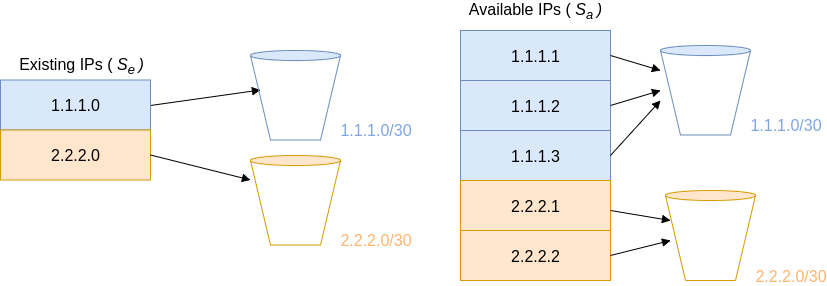
\includegraphics[width=0.8\textwidth]{renders/IpsByBucketSize4Existing.png}
      \caption{Available and Existing IPs Assigned to Buckets of size 4}
      \label{fig:ipsByBucketExisting4}
\end{figure}

Since the total number of IPs required was $t = 7$ and only 4 IPs have been selected, a recursive call is required. As there are still some existing IPs that have not been included, a recursive call is made with the following parameters:
\begin{itemize}
\item{$S'_e = \{2.2.2.0\}$}
\item{$S'_a = \{2.2.2.1, 2.2.2.2\}$}
\item{$t' = 3$}
\end{itemize}

As $t'=3$, the next bucket size will be $b' = 2$ (the highest integral power of 2 smaller than $t'$). Thus, the IPs will be assigned to buckets of size 2, as shown in \reffig{fig:ipsByBucketExisting2}.

The algorithm will then proceed as follows:
\begin{itemize}
\item{Examine the remaining existing ($S'_{e_i}$) and available ($S'_{a_i}$) IP buckets in pairs}
\begin{itemize}
\item{Calculate $b*'_i$ for $2.2.2.0/31$ as per \refeq{eq:ipsToFillBucket}, yielding 1}
\item{Add $2.2.2.0/31$ to $S_c$ as $b*'_i = |S'_{a_i}| = 1$} 
\end{itemize}
\end{itemize}

\begin{figure}[H]
      \centering
      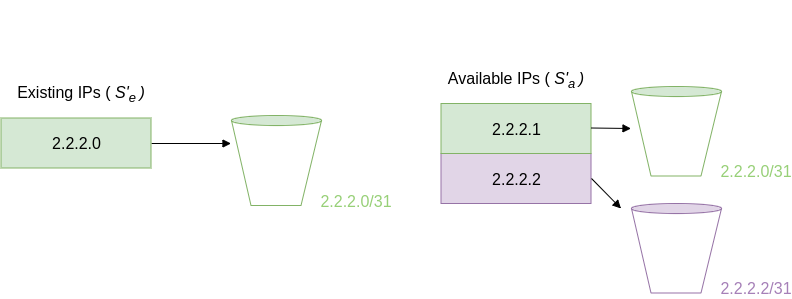
\includegraphics[width=0.8\textwidth]{renders/IpsByBucketSize2Existing.png}
      \caption{Remaining Available and Existing IPs Assigned to Buckets of size 2}
      \label{fig:ipsByBucketExisting2}
\end{figure}

Finally since a total of 7 IPs were required and 6 were selected, a final recursive call is required. However all of the existing IPs are now included in $S_c$, meaning the existing IPs argument for the next recursive call will empty. This means the algorithm falls back to the simple case as described earlier and will choose a random final IP ($2.2.2.2$ in this case). 

There are two enhancements that can be made to the algorithm at this point. The first is a better method for choosing a single IP from the available IP pool. Ideally, the algorithm should choose an \textit{awkward} IP that does not have any free neighboring IPs. Otherwise, the algorithm may break up valuable CIDR blocks by choosing randomly. This is described in \refapp{appendix:smartSingleIP}. 

The other enhancement applies only to the case where the existing set of IPs is non empty. The previously described method of choosing the highest integral power of 2 that is less than $t$ for the initial bucket size only makes sense for the case $S_e = \{\}$. For example, given $S_e = \{1.1.1.0, 2.2.2.0\}$ and $t = 4$, the algorithm must choose two IPs. The described method would suggest starting with a bucket size of $b=4$. However it would be impossible to generate a CIDR block of size 4 given the existing IPs and a choice of only two IPs. An extension to the algorithm to handle choosing the optimum starting bucket size is outlined in \refapp{appendix:smartInitBucket}. 

Finally, the source code for the algorithm is given in \refapp{appendix:algSourceCode}

\subsection{Unit Testing the Algorithm}
The final step in the development was to write extensive unit tests to ensure the algorithm operates as expected. Unit testing is an critical part of the software development process at HubSpot and engineers are always encouraged to write code which is as unit testable as possible. As the code is essentially a number of static utility functions, unit testing is quite simple and does not require mocking any complex objects.  

The initial task was to come up with an example state to test the algorithm with. The example state contains the set of available IP addresses $S_a$ and the set of existing IP addresses $S_e$. These should be chosen in such a way that all code paths of the algorithm are seen at some point or another when running the tests. This requires some consideration as for what is contained in $S_a$ and $S_e$, as well as the total number of IPs required, $t$, for each of the test cases.

As a starting point, the following sets of IPs were chosen for the default state (this can be changed on a per test basis of course):

\begin{equation}\label{eq:initialState}
\begin{gathered}
S_a = \{1.1.1.2, 1.1.1.3, 1.1.1.4, 1.1.1.5, 1.1.1.6, 1.1.1.7, 1.1.1.8, 1.1.1.9\} \\
S_e = \{1.1.1.0, 1.1.1.1\}
\end{gathered}
\end{equation}

Initially however, tests were written for the simplified case where $S_e = \{\}$. The following tests were then implemented:

\begin{itemize}
\item{The algorithm should choose contiguous blocks when available}
      \begin{itemize}
      \item{This was tested by simply requesting that 4 IPs be selected from $S_a$ and ensuring that the resulting set was $\{1.1.1.4/30\}$.}
      \end{itemize}
\item{The algorithm should find contiguous blocks of IPs when a single IP will be left over}
      \begin{itemize}
      \item{This was tested by requesting that 5 IPs be selected from $S_a$}
      \item{The resulting set should contain the block of 4 IP addresses ($1.1.1.4/30$) and a single other IP}
      \item{This test was added to ensure that the algorithm still selected a block of four instead of trying to find several blocks of 2}
      \end{itemize}
\item{The algorithm should find contiguous IPs recursively}
      \begin{itemize}
      \item{This was tested by requesting that 6 IPs be selected from $S_a$}
      \item{The resulting set should contain the block of 4 IP addresses ($1.1.1.4/30$) as before, but should critically select the $1.1.1.2/31$ block for the remaining 2 IP addresses}
      \item{This test was sufficient to assume the algorithm would recursively select CIDR blocks at lower block sizes when available}
      \end{itemize}
\item{The algorithm should always return the correct number of IP addresses}
      \begin{itemize}
      \item{This test was implemented by repeatedly invoking the algorithm with $t$ running from $1$ to $|S_a|$}
      \end{itemize}
\end{itemize}

These tests were sufficient for the simple case where $S_e = \{\}$ and the algorithm was then tested using the more complex case. The following tests were implemented in order to ensure correctness of the algorithm:

\begin{itemize}
\item{The algorithm should find contiguous blocks when provided with existing IP addresses}
      \begin{itemize}
      \item{This was tested by requesting a total of 4 IPs, given the default state as described in \refeq{eq:initialState}}
      \item{The algorithm should then select $\{1.1.1.2/31\}$} so that when unioned with $S_e = \{1.1.1.0/31\}$, the CIDR block $\{1.1.1.0/30\}$  is formed 
      \end{itemize}
\item{The algorithm should always return the correct number of IPs and contain all of the existing IPs}
      \begin{itemize}
      \item{This test was an important test as the algorithm would be useless if it minimized CIDR blocks but didn't guarantee that all of the existing IPs would be present in the resulting set}
      \item{This test was implemented by allowing a variable $i$ to take on values from $1$ to $|S_a|$ and by setting $t = S_e + i$.}
      \item{This essentially repeatedly runs the algorithm, requesting each possible value from the minimum number of new IPs (1), to the maximum number of new IPs (the number of available IPs)}
      \item{At each iteration, the returned set was checked to ensure the correct number of IPs was returned and that all of the existing IPs were contained in that set.}
      \end{itemize}
\item{The algorithm was also tested to ensure it would look for contiguous blocks both above and below (in the IP address space) the existing IPs provided in order to try and find CIDR blocks}
      \begin{itemize}
      \item{This was tested by requesting a total of 2 IPs and setting $S_e = \{1.1.1.3\}$}
      \item{This tested that the algorithm would find CIDR blocks below the existing IPs provided}
      \item{The returned set should be $1.1.1.2/31$, indicating the algorithm correctly searches below the provided existing IPs}
      \item{A similar test was written where $S_e = {1.1.1.2}$ and the algorithm correctly returned $1.1.1.2/31$ indicating that it also looks above the provided existing IP addresses for CIDR blocks}
      \end{itemize}
\item{The algorithm should find CIDR blocks with existing IP addresses that cause a single IP to be left over}
      \begin{itemize}
      \item{This was tested by requesting a total of 9 IPs using the default state as shown in \refeq{eq:initialState}}
      \item{The resulting set should contain the CIDR block of 8 IPs ($1.1.1.0/29$) and the remaining extra IP ($1.1.1.9$)}
      \end{itemize}
\item{The algorithm should return already grouped existing IPs}
      \begin{itemize}
      \item{It is essentially impossible to break up a CIDR block contained inside the set of existing IP addresses, but this test was added to ensure the algorithm correctly identified existing CIDR blocks appropriately.}
      \item{A set of existing IPs $S_e = \{2.2.2.0/31\}$ was used along with an the available set of IPs listed in \refeq{eq:initialState} and a total of 4 IPs were requested.}
      \item{The algorithm correctly returned the existing CIDR block as well as another CIDR block of size 2, yielding $\{1.1.1.2/31, 2.2.2.0/31\}$}
      \end{itemize}
\item{The algorithm should handle existing IPs which don't contribute to any CIDR blocks and should fill the remaining number of IPs required with the best CIDR block from the available set of IPs}
      \begin{itemize}
      \item{This was tested by setting $S_e = \{2.2.2.0, 3.3.3.0, 4.4.4.0\}$}, using the set of available IPs shown in \refeq{eq:initialState} and requesting 5 IPs.
      \item{The algorithm should then return the three existing IPs along with a CIDR block of size 2 from the set of available IPs}
      \end{itemize}
\end{itemize}

These tests provided a sufficient amount of coverage to provide confidence in the algorithm and its implementation. Several other tests were implemented which were less specific to the algorithm (such as ensuring user input was validated). The algorithm has been running in a production environment for over 3 months and has helped automate an important step that was previously being performed manually by a support team at HubSpot.   
\chapter{Conclusion}
In conclusion, the internship provided a fantastic insight into how software is developed in an enterprise environment and provided ample opportunity to learn new concepts and extend knowledge on previously studied topics. 

Over the course of the internship, experience was gained working with a variety of new and exciting technologies such as Kafka (\refsec{sec:kafka}) and Hadoop (\refsec{sec:hadoop}). Knowledge gained from previous modules of the course on fundamental computer science principles, problems and techniques (for example immutability, dependency injection, databases and distributed systems) was put into practice and used to deliver industry standard, well tested software that is used millions of times per day in a production environment.

The internship also provided an opportunity to practice and improve upon softer skills such as time management, time estimation for software development tasks, hosting and contributing to meetings with other engineers and reviewing code submitted by teammates. Although modules aiding in developing these fundamental industry skills are available throughout the MAI program, having the chance to use these skills on a daily basis provides an excellent means of improving these skills in a real enterprise environment.


\bibliographystyle{unsrtnat}
\bibliography{bibliography}

\renewcommand{\thechapter}{A\arabic{chapter}}
\begin{appendices}

\chapter{Source Code for DNS Management System}
\label{appendix:dnsManagement}
\lstinputlisting[
  caption={The DnsRecordBuilder interface},
  label={lst:dnsRecordBuilder},
  style=javaStyle
  ]{code/tasks_undertaken/dns_management/DnsRecordBuilder.java}

\lstinputlisting[
  caption={Apply \java{DnsRecordBuilder}s and find records that need updating.},
  label={lst:recordBuilderApplier},
  style=javaStyle
  ]{code/tasks_undertaken/dns_management/DnsRecordBuilderApplier.java}

\lstinputlisting[
  caption={A simplified DNS sync job implementation},
  label={lst:dnsSyncJob},
  style=javaStyle
  ]{code/tasks_undertaken/dns_management/DnsSyncJob.java}

\chapter{Intelligently Choosing a Single IP from the Available Pool}
\label{appendix:smartSingleIP}
Content content..

\chapter{Intelligently Calculating the Initial Bucket Size}
\label{appendix:smartInitBucket}
Content content

\chapter{Source Code for the CIDR Minimization Algorithm}
\label{appendix:algSourceCode}
Content content



\end{appendices}

\end{document}